\documentclass[11pt,a4paper]{article}
\usepackage{fullpage}
\usepackage{cite} 
\usepackage[breaklinks,colorlinks,urlcolor=blue,citecolor=blue,linkcolor=blue]{hyperref} 	%Hyperlinks everywhere!
\usepackage{natbib}
\usepackage{graphicx}

\begin{document}

\title{Project Plan - Constraining the Hemispherical Structure in the Hidden Layer At the Top of the Earth's Inner Core}
\author{David Stansby \\ ds598@gmail.com }
\maketitle

\begin{abstract}
Since it's discovery in 1936, the Earth's Inner Core has been well documented by both body wave and normal mode studies. However, one area where properties are not yet well measured is the top of the inner core. This region is of particular interest as it is thought that as the outer core freezes onto the inner core it's history is encoded in the properties of the frozen material.

This project will use various techniques centred around seismic body wave analysis in order to attempt to measure the top 20km of the inner core. It is hoped that a detailed regional velocity structure can be mapped using these techniques. If this is not possible, the project will still be able to quantify to what extent these techniques are applicable, thus providing a useful feasibility study.
\end{abstract}

\section{Scientific Motivation}
The inner core of the Earth is a solid sphere, surrounded by a liquid outer core. It was first discovered by Inge Lehmann in 1936, who used the existence of P wave arrivals within the P wave shadow zone to infer a solid-liquid boundary lying within the Core-Mantle Boundary (CMB). Over the following 80 years large progress has been made on measuring the properties of the inner core.

Of particular interest is the velocity structure; \cite{Deuss2014} gives a brief review of the current state of research into this are. Currently research shows that the the top 80km of the inner core is isotropic, with deeper parts having $\sim 3\% $ anisotropy. Studies have also revealed that the inner core is split into two hemispheres, a western and an eastern one, each of which have differing attenuation and anisotropy properties.

So far only large scale velocity structures have been measured. In particular, both the smaller scale regional structure of the top 20km of the inner core and the structure of the hemisphere boundary at this depth are currently poorly measured. The upper inner core is of particular interest as material from the outer core is currently freezing onto it at a rate of around 1mm/year. Modelling performed by \cite{Deguen2009a} shows that the velocity structure of the upper inner core should result from recent processes in the lower upper core, and thus determine the history of the outer core. This in turn could give insights into areas such as how the outer core generates the Earth's magnetic field.

\section{Project Goals}
\label{sec:Goals}
The primary aim of this project is to create a velocity model for the upper 20km of the inner core. In particular we hope to constrain the detailed regional structure, focusing specifically around the hemisphere boundaries. It is hoped that we may be able to locate the position of the boundary at the top of the inner core, extending the results of \cite{Waszek2011b}. This may not be possible due to the limitations of the method described in section \ref{sec:Methodology}, but in this case it will still be useful to produce quantitive results that place limits on the applicability of the considered methodology to the problem in hand.

If time permits, and depending on results in the early stages of the project, other possible questions to answer will be:
\begin{itemize}
	\item Can we quantify the minimum depth for which the velocity structure can be resolved using PKiKP - PKIKP seismic body wave studies?
	\item Are there any other novel techniques that would allow small PKiKP - PKIKP differential travel times to be measured to high accuracy?
	\item Is it possible to distinguish between a sharp or a gradual hemisphere boundary using body wave seismic studies?
\end{itemize}

\section{Project Methodology}
\label{sec:Methodology}
As it is not possible to directly sample the properties of the inner core, the properties must be inferred using seismic waves. Both high frequency seismic body waves and low frequency normal mode studies are used; this project will focus on the use of seismic body waves. 

Properties of the inner core can be measured using the arrival times of two different body seismic waves generated by earthquakes, PKiKP and PKIKP. Figure \ref{fig:RayPaths} (taken from \cite{Waszek2011a}) shows the ray paths for each of these waves. The reference PKiKP wave reflects off the inner core boundary (ICB), whereas the PKIKP wave travels within the inner core. Any differences between the travel times of these two waves is therefore a measure if the inner core structure.

Figure \ref{fig:Seismogram} (taken from \cite{Waszek2011a}) shows an example seismogram with PKiKP and PKIKP arrivals marked on. As the maximum depth that the PKIKP wave travels beneath the ICB is reduced, the differential travel time reduces causing the individual wave packets to overlap, limiting our ability to distinguish them.

\begin{figure}
	\centering
	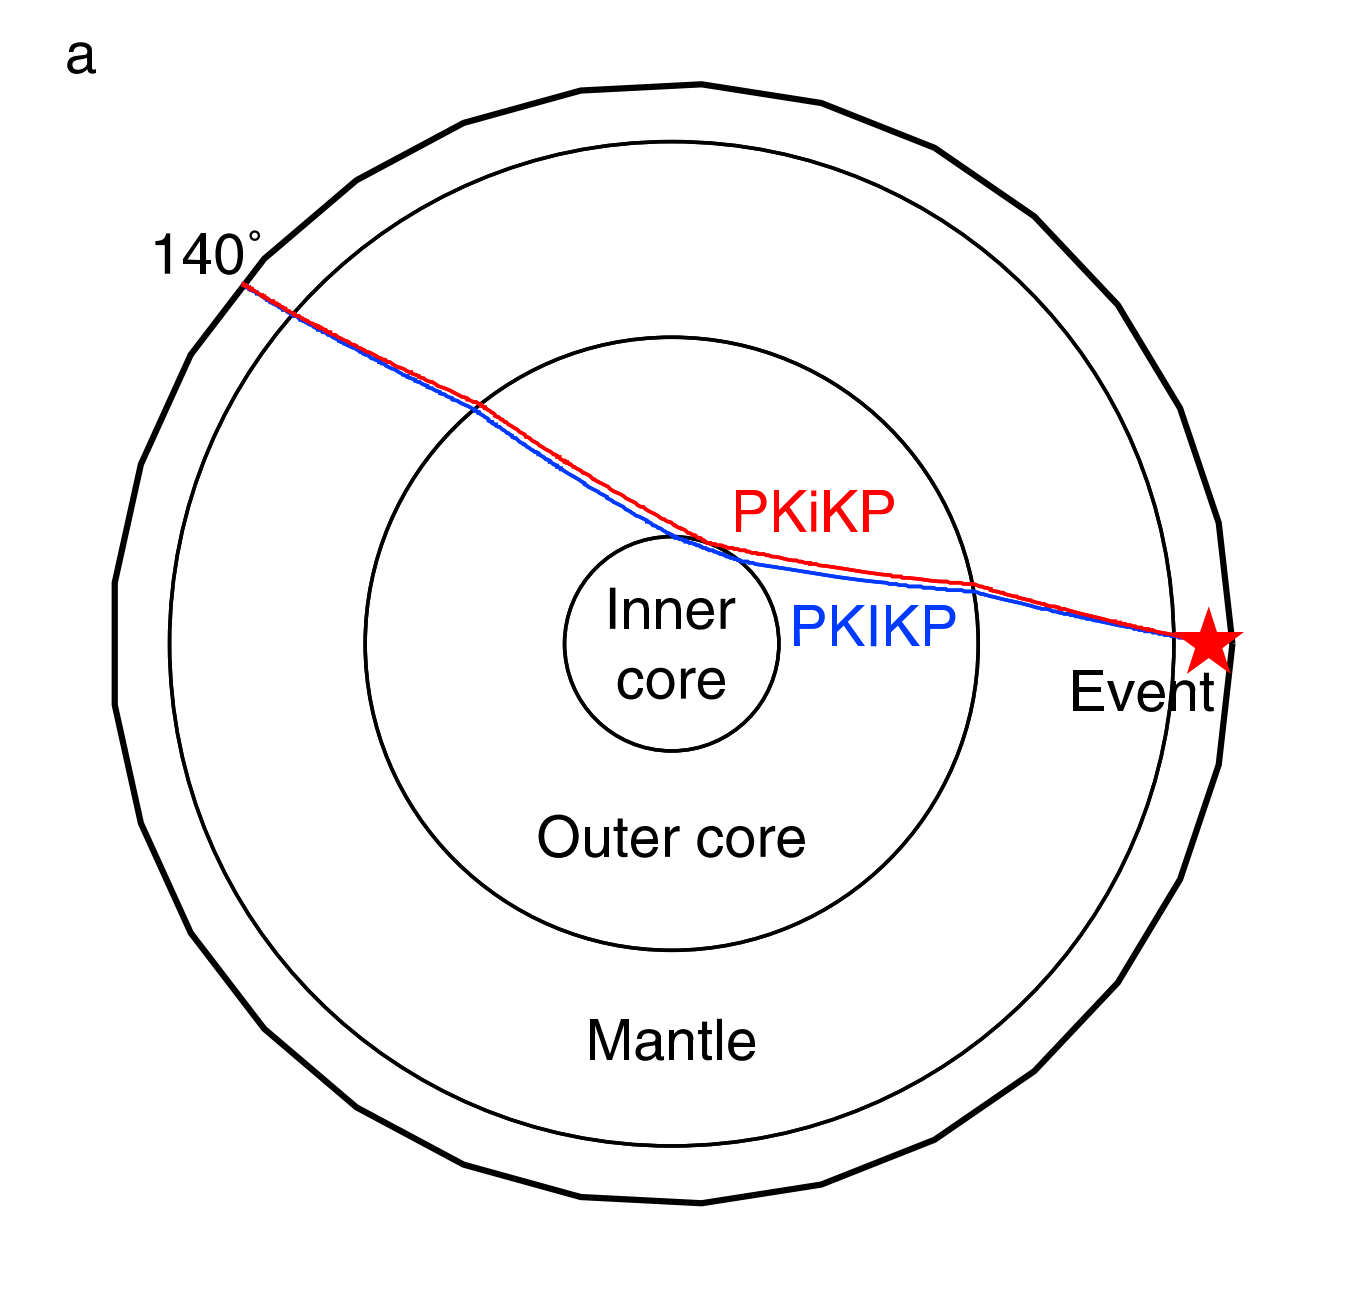
\includegraphics[width=0.5\textwidth]{RayPaths.png}
	\caption{The ray paths for PKiKP and PKIKP seismic body waves. (taken from \cite{Waszek2011a})}
	\label{fig:RayPaths}
\end{figure}

\begin{figure}
	\centering
	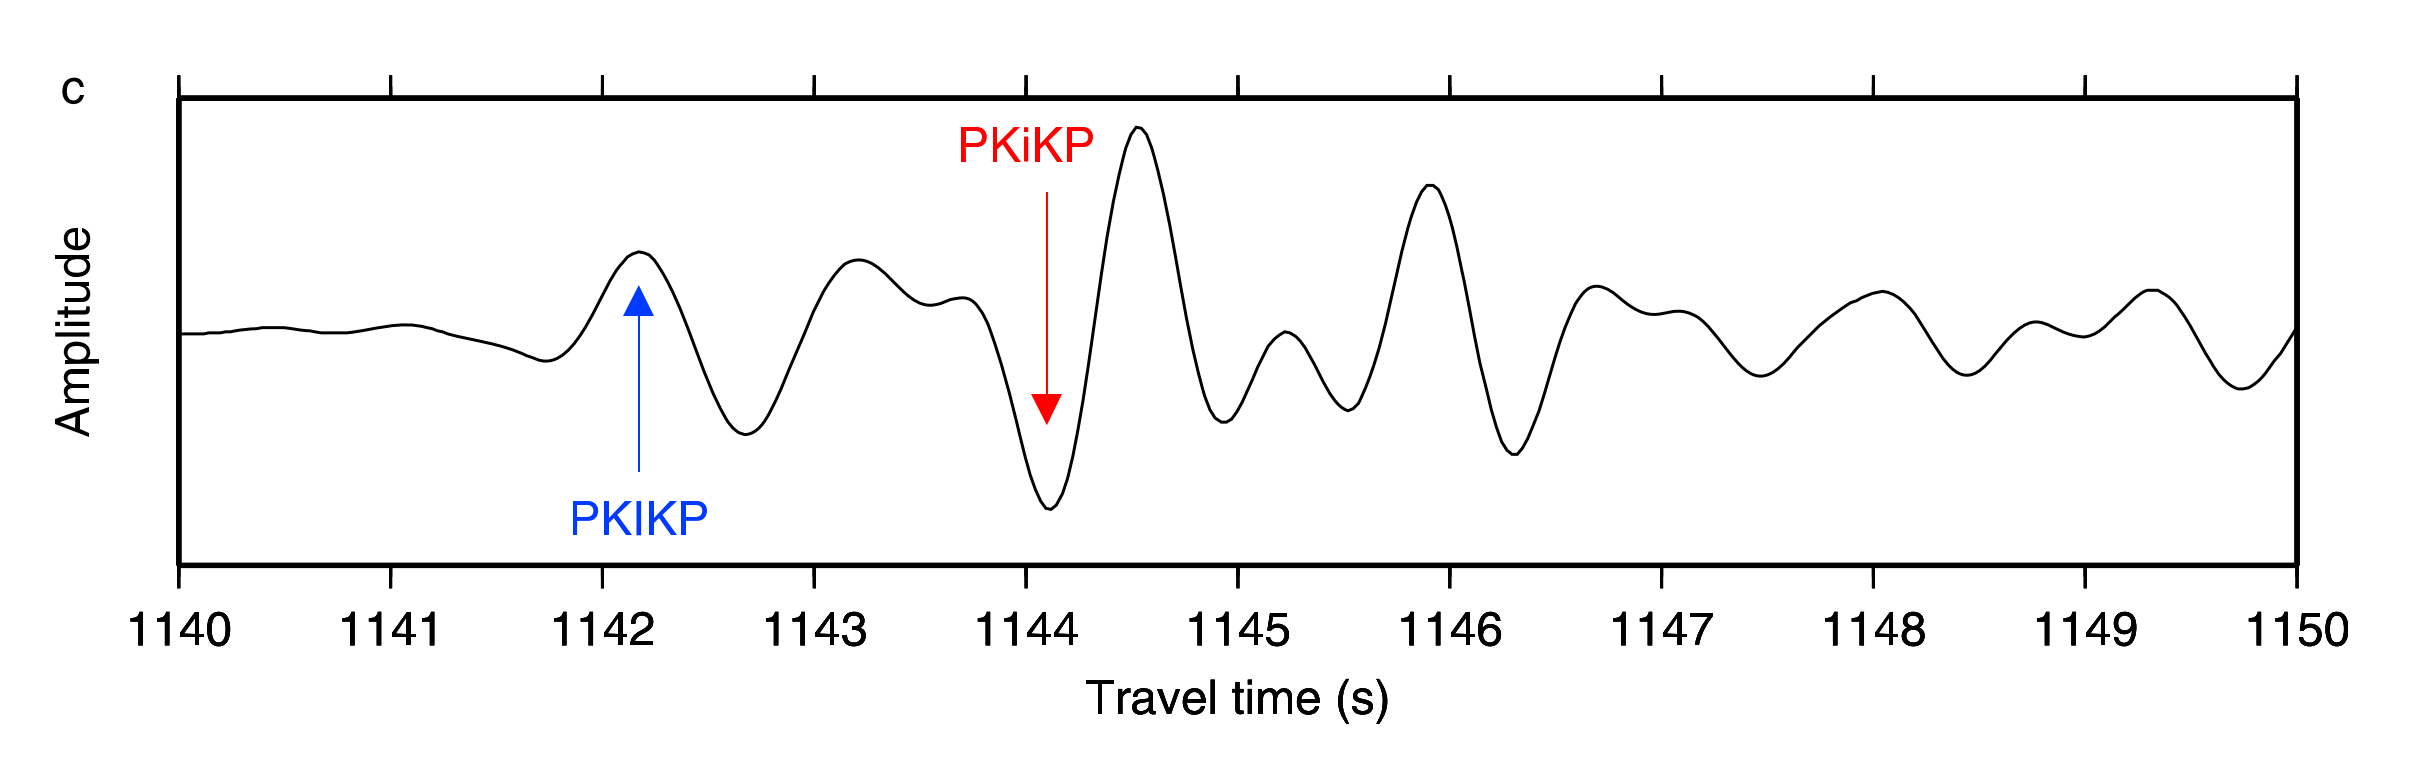
\includegraphics[width=\textwidth]{Seismogram.png}
	\caption{Example seismogram showing identification of PKiKP and PKIKP waves (taken from \cite{Waszek2011a})}
	\label{fig:Seismogram}
\end{figure}



From these seismometer measurements, and with a velocity structure model in place, the differential travel time is defined as

\begin{equation}
	\delta t = (t_{PKiKP} - t_{PKIKP})_{data} - (t_{PKiKP} - t_{PKIKP})_{model}
\end{equation}

This gives a measure of the error along a given ray path from a 1D reference model (eg. \cite{Kennett1995}) that assumes velocity is only a function or radial distance; a high $\delta t$ value indicates an anomalously high velocity along the ray path and vice versa. Plotting $\delta t$ values as a function of depth and longitude will allow us to reveal any anomalous velocity structure\footnote{This is the methodology employed in \cite{Waszek2011a} in order to map the hemispherical boundary.}.

Alternatively, when making velocity models we will seek to make $\delta t$ values as close to zero as possible for all ray paths. This will be achieved by using the WKBJ program to model ray paths, and allow us to construct a velocity model which matches the data. We can do this for a variety of turning depths and longitudes in order to create a 2D velocity model. Once this velocity model is in place it can then be tested using the much more sophisticated Axisem program (\cite{Nissen-Meyer2014}). This will allow synthetic seismograms to be created for our model, allowing comparison with real world data that did not play a part in creating the model, thus ensuring a good test of the model.



\section{Project Plan}

\begin{enumerate}
	\item Initially we will take 5 earthquakes, and download the real world seismic data from a number of monitoring stations for each quake. This will allow the construction of a velocity model for the range of longitudes and depths that the monitoring stations cover, using the WKBJ program to perform waveform modelling.
	\item Once a non-1D velocity model has been calculated, it will then be fed into the much more advanced Axisem program. This will allow synthetic seismograms to be calculated for any phase and any location on the earth's surface.
	\item The synthetic seismograms can then be compared to the real data in order to test the new model.
	\item The remainder of the project will remain flexible, depending on the time remaining and the results of the previous steps. Suggested further areas to investigate are given in section \ref{sec:Goals}
\end{enumerate}

\bibliographystyle{yahapj}
\bibliography{/Users/dstansby/Physics/Papers/library}


\end{document}